\chapter{État de l'art\label{sec:state_of_the_art}}
Il est hélas impossible de réaliser un état de l'art complet sur le
\raytracing{}\ car cela nécessiterais des mois de recherches et mériterait un
papier complet\footnote{À ce sujet, je vous invite à consulter
\cite{Wald01stateof}}. Nous pouvons cependant retracer les grandes dates de
cette technologie et tenter d'en apercevoir les perspectives. 

\remark{Cette étude est principalement basé sur \cite{webWayne03} et
\cite{webWayne06}.}

\section{Découverte} 
C'est en 1968 (!!!) que \tsc{Arthur} et \tsc{LaFortune} publient
\cite{Lafortune93} dans lequel ils abordent la possibilité d'effectuer un
rendu en calculant l'intersection des objets avec la lumière --- en
l'occurrence un ensemble de rayons virtuels. 

Le \eng{ray casting}\ est né mais il faudra attendre un dizaine d'années avant
que soit publié un algorithme capable de surpasser la \eng{rasterization} (\cf
\ref{sec:rasterization}) en terme de qualité. En effet, le \eng{ray casting}
se contente de lancer un rayon primaire afin de déterminer s'il y a
intersection ou non sans pour autant pousser la calcul plus loin.

\section{La révolution}
Le \raytracing{}\ tel que nous le connaissons aujourd'hui fait ses premières
armes dans \cite{Whitted1980}. Les auteurs y introduisent la notion de rayons
secondaires crées à chaque intersection avec un objet. Ainsi apparait la
possibilité d'effectuer le rendu de phénomènes tels que la réflexion et la
réfraction. \tsc{Whitted} souligne par ailleurs que la gestion de
l'anti-aliasing est totalement intégré au pipeline de rendu. C'est une
caractéristique importante car aujourd'hui encore, les techniques
d'anti-aliasing ``coûtent chère en calcul''.

La \tsl{fig.}\ \ref{fig:firstRendering} présente un des rendus de
\cite{Whitted1980} où nous pouvons constater que déjà à l'époque, la qualité
du \raytracing{} était incomparable à celle de la rasterisation.
\begin{figure}
\begin{center}
  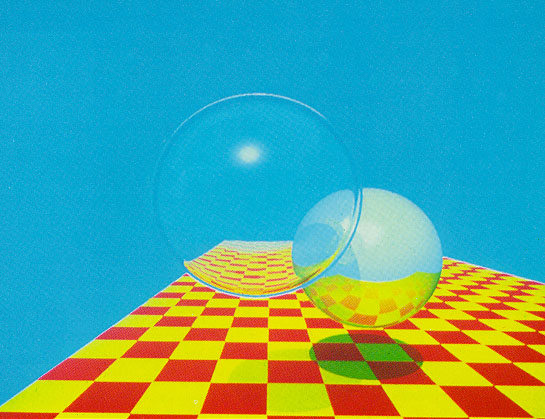
\includegraphics[width=.8\textwidth]{img/1980_Raytracing.jpg}
  \caption{Un rendu de \cite{Whitted1980}\label{fig:firstRendering}}
\end{center}
\end{figure}

Très vite après cette publication, de nombreuses améliorations ont été
apportées à l'algorithme. On peut citer notamment les ombres floues (ou
douces), le \gls{jittering}, le \gls{motion_blur} ou encore
l'\gls{adaptative_sampling}.

\section{Bi-directional path tracing}
La seconde révolution du domaine tire ses origine dans l'avènement du
\eng{bi-directionnal path tracing}. Le terme fait référence au fait qu'au
lieux de simplement considérer les rayons partant de la caméra pour aller
jusqu'à la scène (\tsl{backward rays}), l'algorithme considère une équation
intégrant les rayons partant des différentes sources de lumière (qui, nous le
verrons, peuvent être tous les objets de la scène). C'est aujourd'hui la plus
grande piste de recherche pour améliorer le rendu de scènes complexes et si la
théorie est déjà très évoluée, de gros travaux d'optimisation restent à
effectuer.

Étudions brièvement 2 des approches les plus utilisées.

\subsection{Radiosity\label{sec:radiosity}}
La radiosité est une méthode de résolution de l'équation \ref{eq:radiosity} (à
titre d'illustration...).
\begin{figure}[h]
  $$B(x)\, dA = E(x) \, dA +\rho(x) \, dA \int_{S}B(x') \frac{1}{\pi r^2}
  \cos\theta_x\cos\theta_{x'} \cdot \mathrm{Vis}(x,x') \,\mathrm dA'$$
  où \begin{itemize}
    \item $B(x)dA$ est l'énergie totale de la zone en question,
    \item $E(x)$ son énergie émise,
    \item $\rho (x)$ sa réflectivité,
    \item $r$ la distance entre $x$ et $x'$,
    \item $Vis$ une fonction binaire valant 1 si $x$ et visible de $x'$ et 0
      sinon.
  \end{itemize}
  \caption{Équation de transfert de
  lumière.\label{eq:radiosity}\cite{wikipediaRadiosity}}
\end{figure}

Cette équation, tirée des transfert de chaleurs, s'applique très bien aux
transferts de lumière d'une surface à une autre. Les
\tsl{fig.\ref{fig:withoutGI} et \ref{fig:withGI}} montrent bien la différence
que l'illumination globale apporte au réalisme de la scène. 

Alors que sans illumination globale, les murs gardent leur teinte d'origine,
l'ajout de l'intégration de l'algorithme de radiosité transfert de la couleur
du mur vert (invisible sur l'image) sur le mur du fond. 

\begin{figure}[h]
  \begin{center}
    \subfigure[CornelBox sans illumination globale.\label{fig:withoutGI}]
    {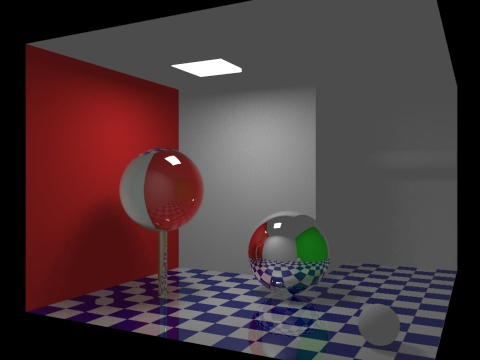
\includegraphics[width=.4\textwidth]{img/withoutGI}}
    \subfigure[CornelBox avec illumination globale.\label{fig:withGI}]
    {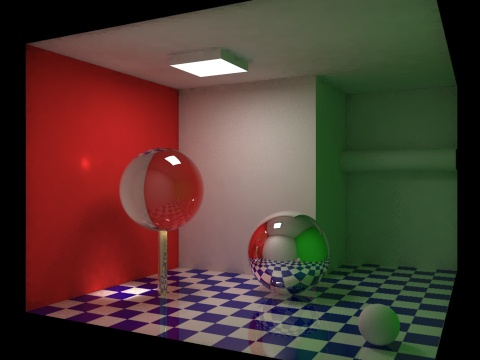
\includegraphics[width=.4\textwidth]{img/withGI}}
  \end{center}
\end{figure}

Plus concrètement, l'algorithme se contente de lancer des rayons depuis les
différentes sources lumineuses et calcule les rebonds de ceux-ci. Évidemment,
l'émission des rayons n'est pas totalement aléatoire et suit des lois de
distributions. À chaque nouvelle intersection, la contribution de la source
est ajoutée à l'image. 

\remark{Cette méthode à l'avantage d'être relativement simple à implémenter.}

\subsection{Photon mapping}
Une autre méthode très efficace d'illumination globale est le \tsl{photon
mapping}. Contrairement à la radiosité qui ajoute la contribution des rayons
par itération, le \tsl{photon mapping}\ crée une cartographie des photons
lancés depuis la source lumineuse jusqu'aux objets de la scène. À chaque
collision, le photon est soit absorbé, soit réfléchi, soit les deux.

Cette technique permet de reproduire le phénomène de caustique, qui est une
concentration de photons dans une zone de l'espace comme le montre la
\tsl{fig.\ref{fig:caustic}}.

\begin{figure}
\begin{center}
  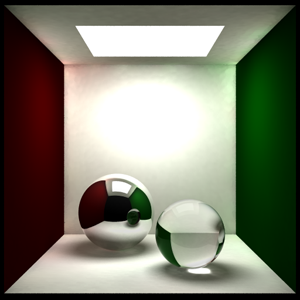
\includegraphics[width=.8\textwidth]{img/caustic}
  \caption{Un exemple de caustique (sous la sphère de
  droite).\label{fig:caustic}}
\end{center}
\end{figure}

Cette méthode est cependant plus difficile à implémenter puisqu'elle nécessite
des structures accélératrice comme les Kd-Tree afin de pouvoir ``compter'' le
nombre de photons dans une certaine zone de l'espace de manière efficace.

\remark{Ces deux approches forment la base des techniques utilisées mais
évidemment, il existe de nombreuses variantes, que ce soit au niveau des
structures de donnée, des distribution statistique, des équations de rendu,
\etc dont la plus important est le \tsl{final gathering}.}

\subsection{Demain ?}
Si l'avenir du \raytracing{}\ dans l'informatique de tous les jours est
certain, il faudra attendre que les CPU puissent calculer efficacement les
images pour voir cette technique remplacer la rasterisation.. Cela nécessite
donc du nouveau matériel et des algorithmes encore plus performant.\\

Il est cependant déjà possible de faire du \raytracing{}\ temps réel sur des
\glspl{GPU} ``de bureau'' grâce à des projets comme \tsl{OpenRT}\ ou
\tsl{Optix}.
